
\section*{Supplement}

\setcounter{figure}{0}
\makeatletter 
\renewcommand{\thefigure}{S\@arabic\c@figure}
\makeatother

\begin{figure}
  \begin{center}
    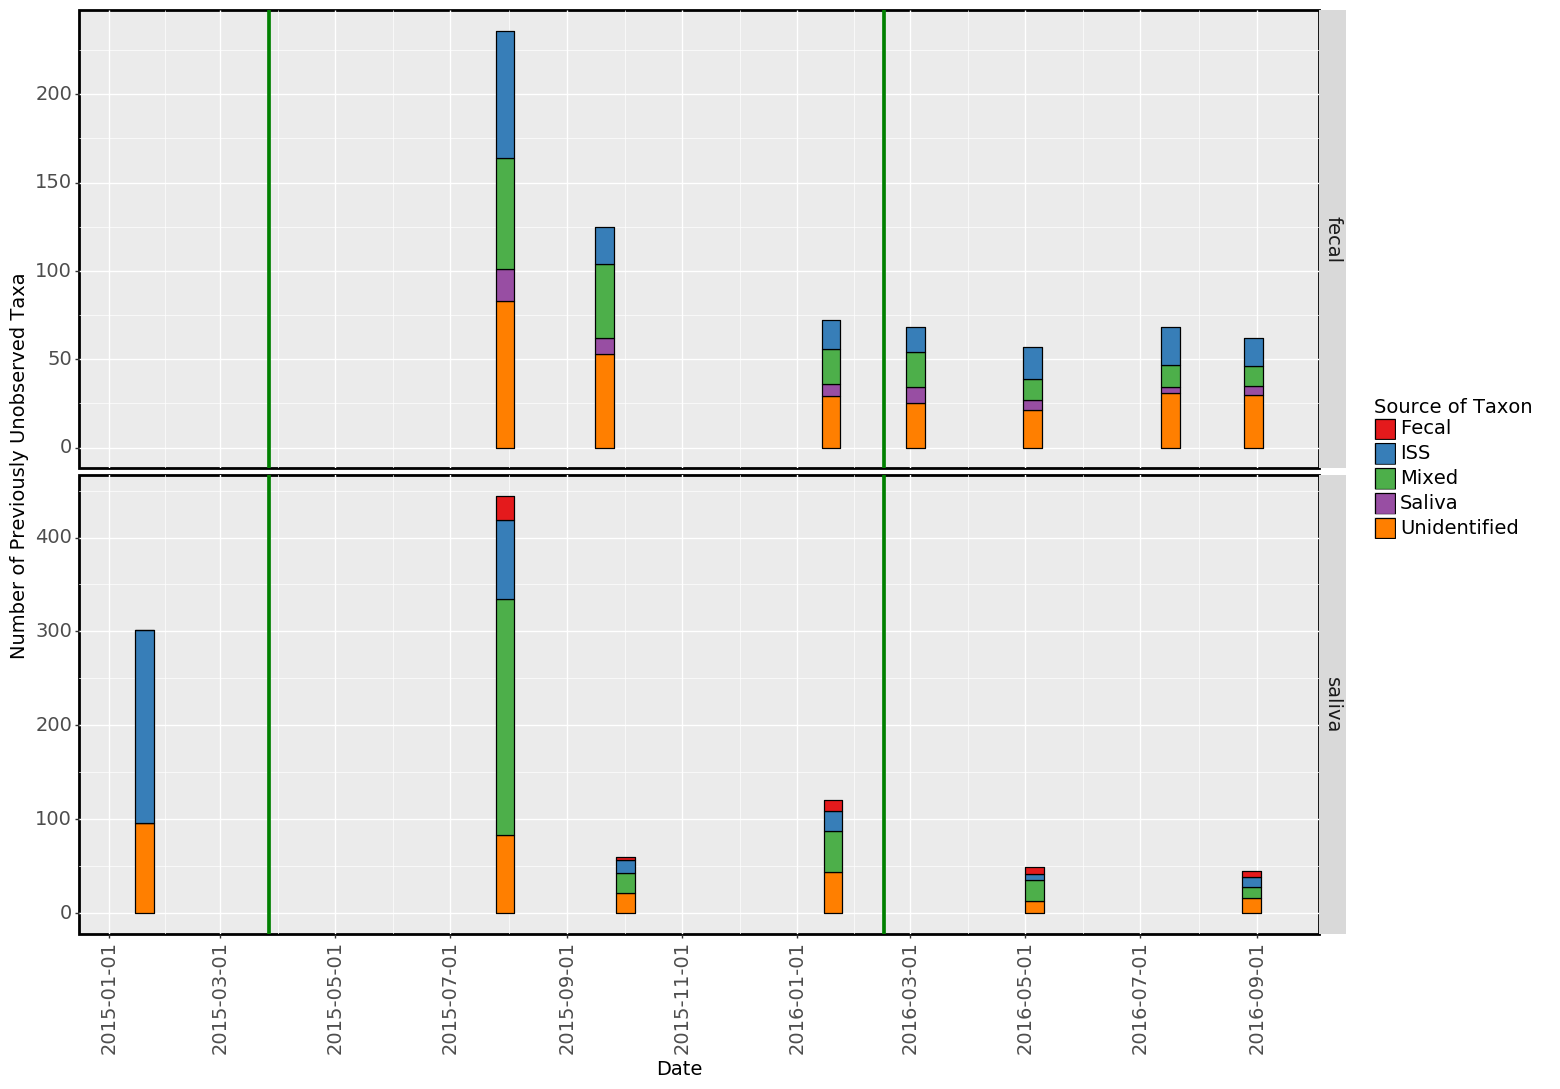
\includegraphics[width=0.99\textwidth]{figs/hr_taxa_sources.png}
%	\vspace{-20pt}
	\caption{\small{
	    This plot shows the number of taxa at each time point that were not observed at any previous timepoint for fecal and saliva samples from HR. The colors indicate the likely source of the new taxon if it was found previously in the saliva (for fecal samples, vice versa for saliva samples), the ISS, both (Mixed), or neither.
	}}
    \label{fig:hrtaxasource}
  \end{center}
%  \vspace{-20pt}
 % \vspace{1pt}
\end{figure}

\begin{figure}
  \begin{center}
    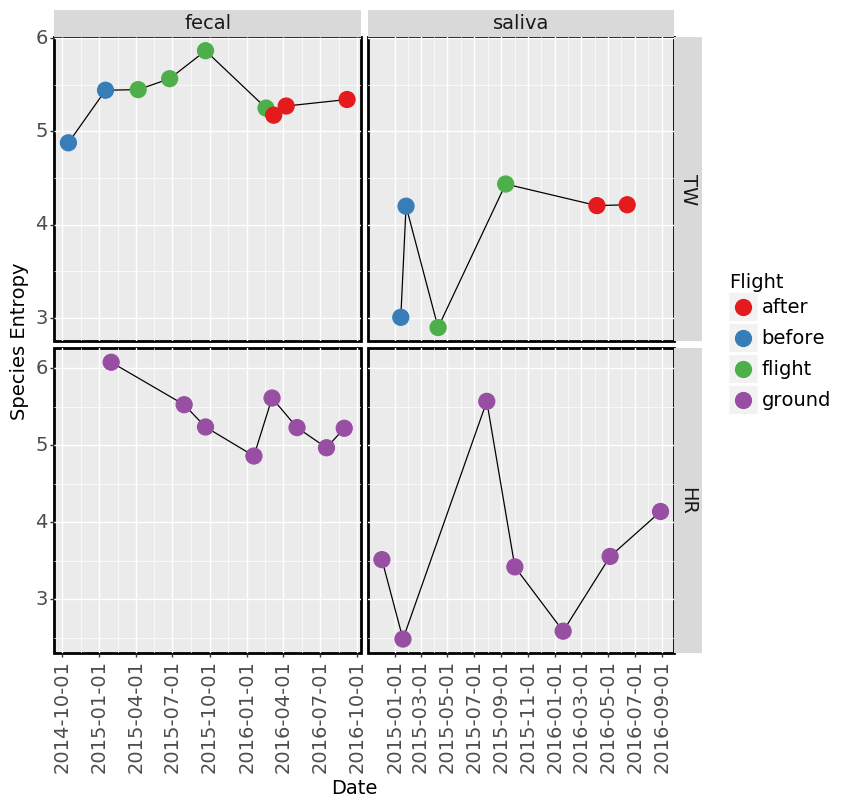
\includegraphics[width=0.99\textwidth]{figs/species_diversity.png}
%	\vspace{-20pt}
	\caption{\small{
	    Vertical shows species entropy (Shannon entropy of species relative abundances) for sample types in both twins.
	}}
    \label{fig:taxadiv}
  \end{center}
%  \vspace{-20pt}
 % \vspace{1pt}
\end{figure}

\begin{figure}
  \begin{center}
    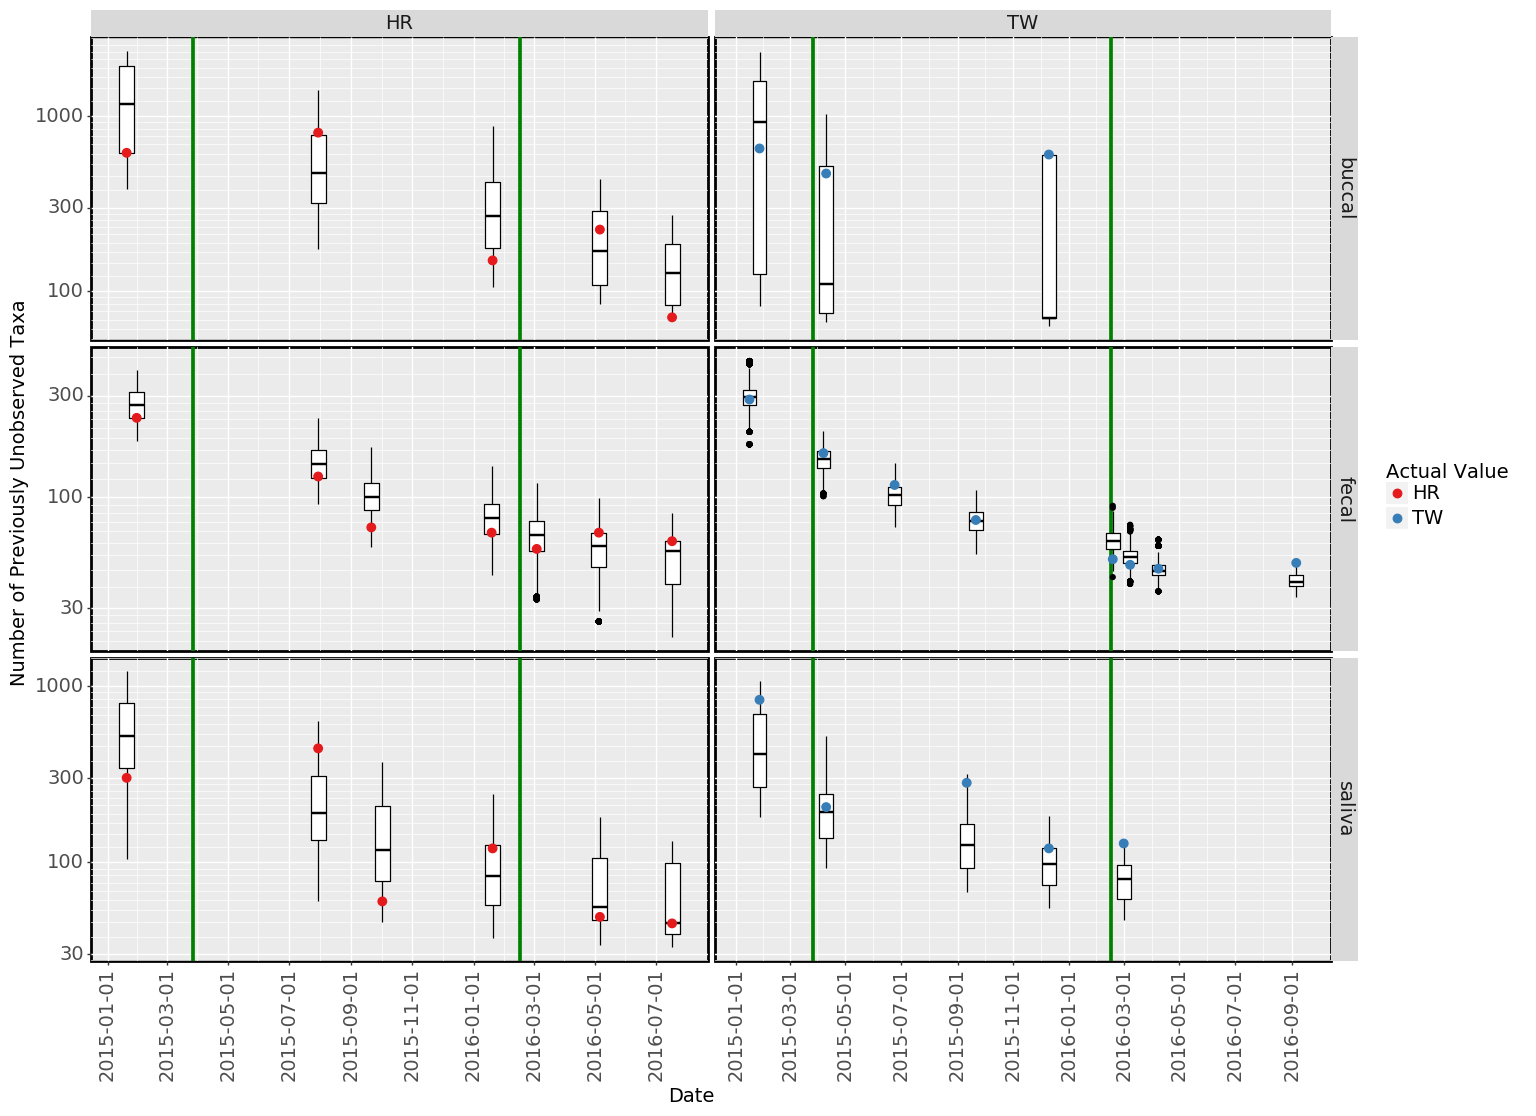
\includegraphics[width=0.99\textwidth]{figs/twins_taxa_flux.png}
%	\vspace{-20pt}
	\caption{\small{
	    This plot shows the number of taxa at each time point that were not observed at any previous timepoint. The first timepoint is omitted from the plot since no taxa had been previously observed. Boxplots indicate an artificial reference distribution generated by randomly permuting timestamps. Red and blue dots indicate actual values.
	}}
    \label{fig:taxaflux}
  \end{center}
%  \vspace{-20pt}
 % \vspace{1pt}
\end{figure}

\begin{figure}
  \begin{center}
    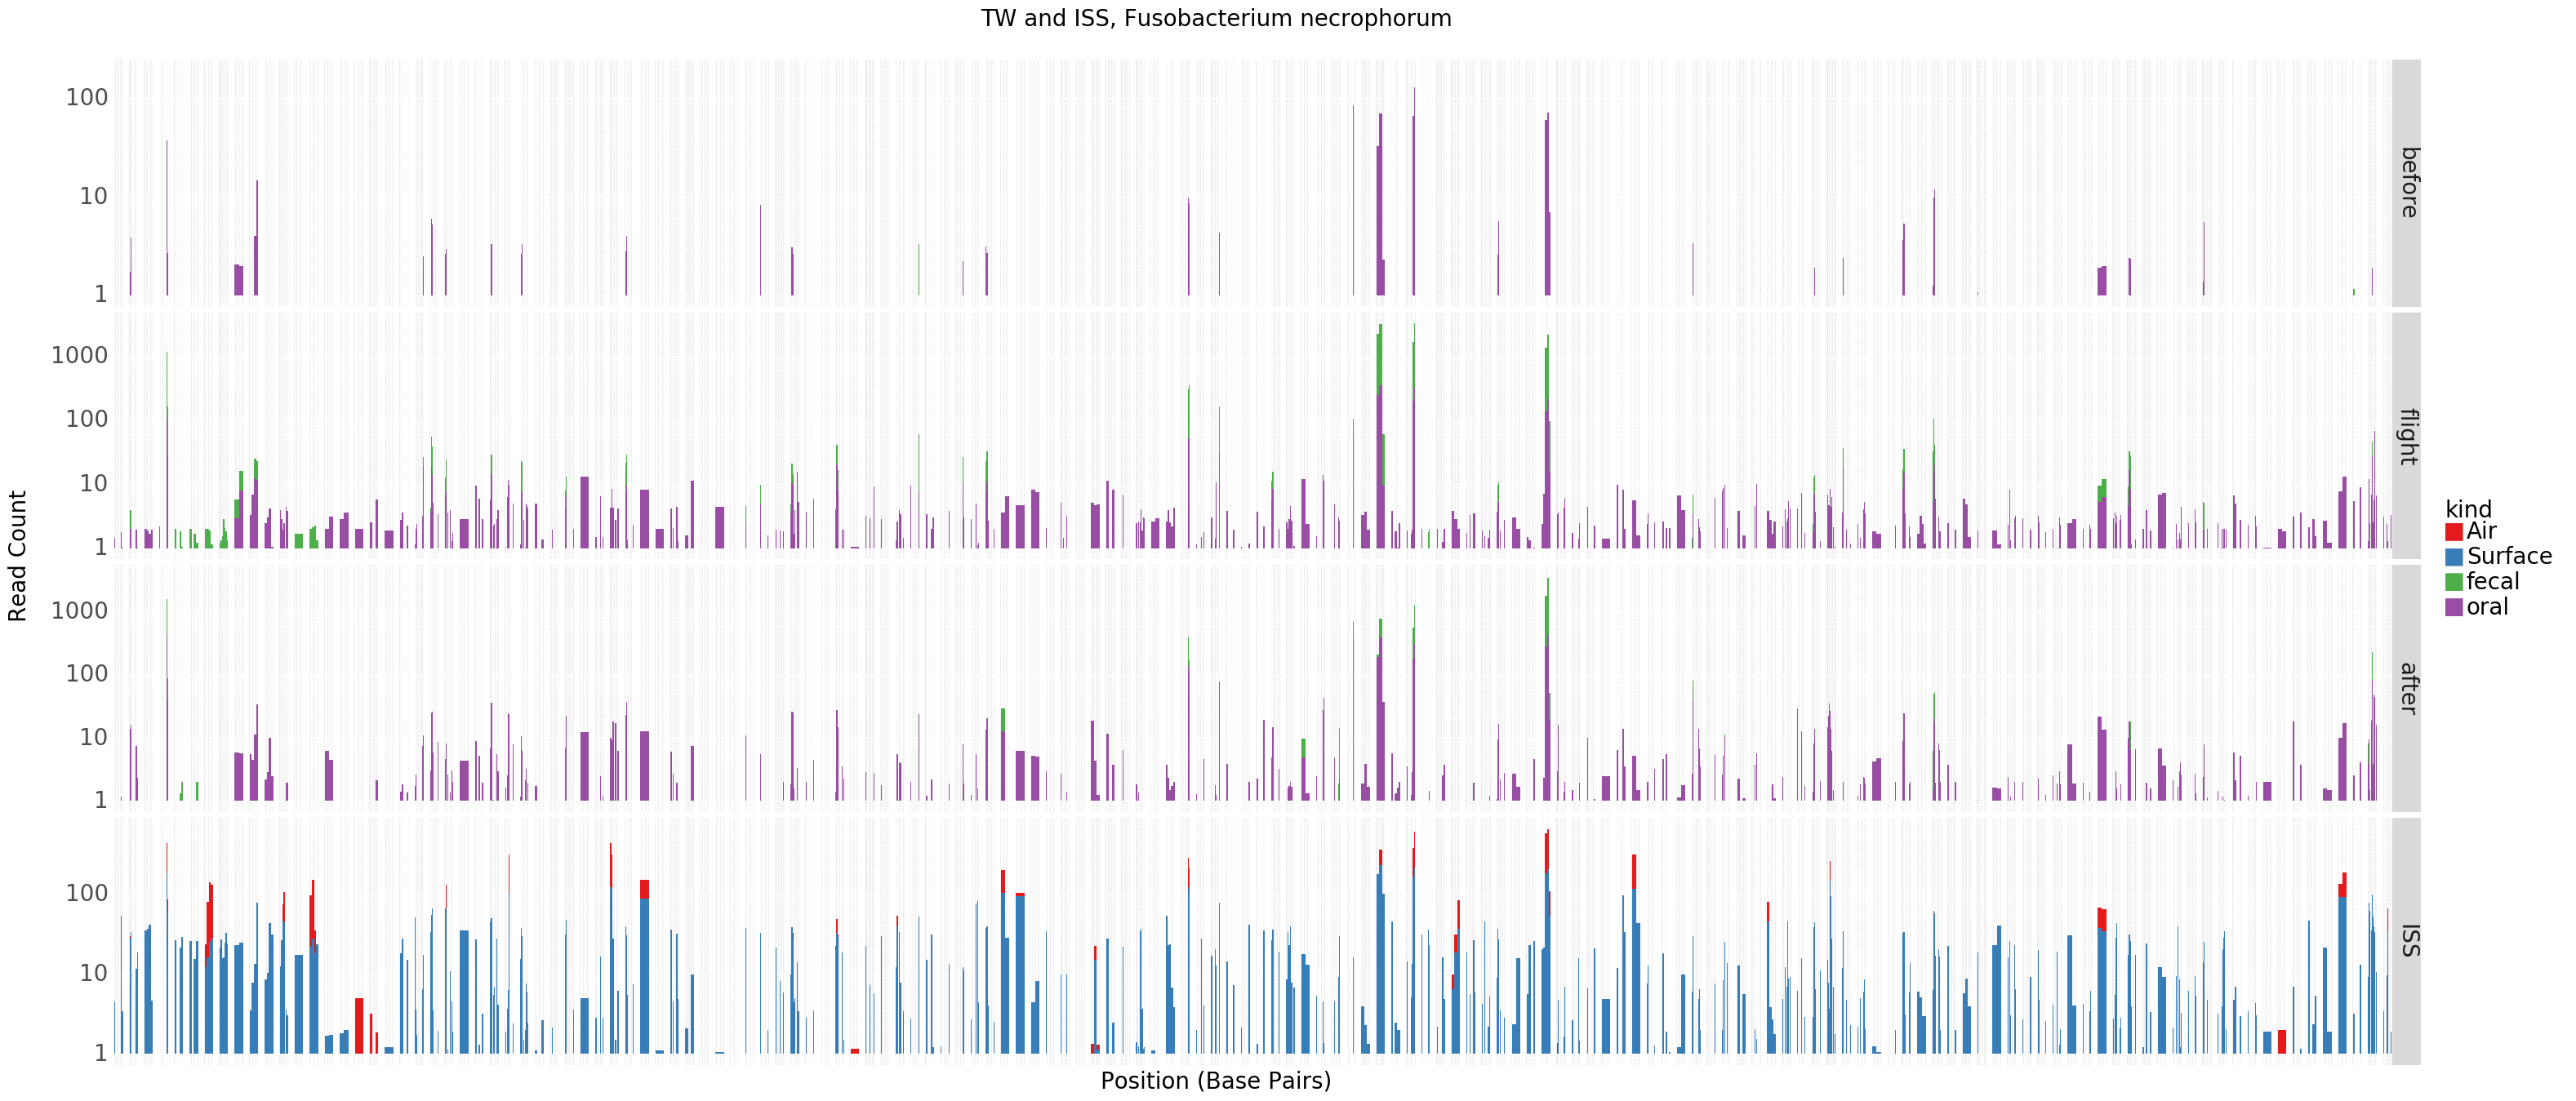
\includegraphics[width=0.99\textwidth]{figs/f_necro_read_recruit.png}
%	\vspace{-20pt}
	\caption{\small{
	    Rows show consolidated samples from before, during and after flight (or from the ISS at any point) from TW. Columns represent all available contigs for taxon. Colored bars represent 100bp covered, on average, at the specified read depth. A number of contigs are only covered in TW during and after flight.
	}}
    \label{fig:fnecro}
  \end{center}
%  \vspace{-20pt}
 % \vspace{1pt}
\end{figure}


